\chapter{Best practices}
Fino ad ora ci siamo concentrati sulla comprensione dell'algoritmo di backpropagation. Nel seguito introdurremo un insieme di tecniche che possono essere utilizzate per migliorare il modo con cui la rete impara.
\section{Il problema dello Slow Learning}
Le reti basate sulle sigmoidi con una quadratic loss function sono spesso molto lente.
\begin{figure}[h]
    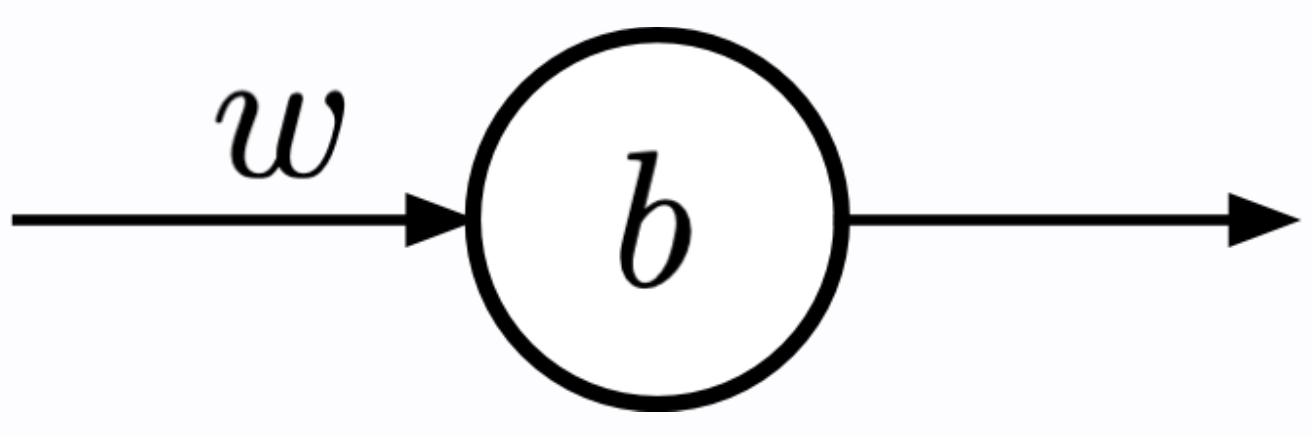
\includegraphics[scale=.5]{images/best_practices/slow_net.png}
    \centering
\end{figure}



Per capire il motivo, consideriamo una rete neurale molto semplice (quella in figura) e consideriamo il learning problem che tratta di mappare $1$ in input in $0$ in output. In questo esempio, $C$ è il costo quadratico e l'unità di output è una sigmoide.
\newpage
\begin{figure}[h]
    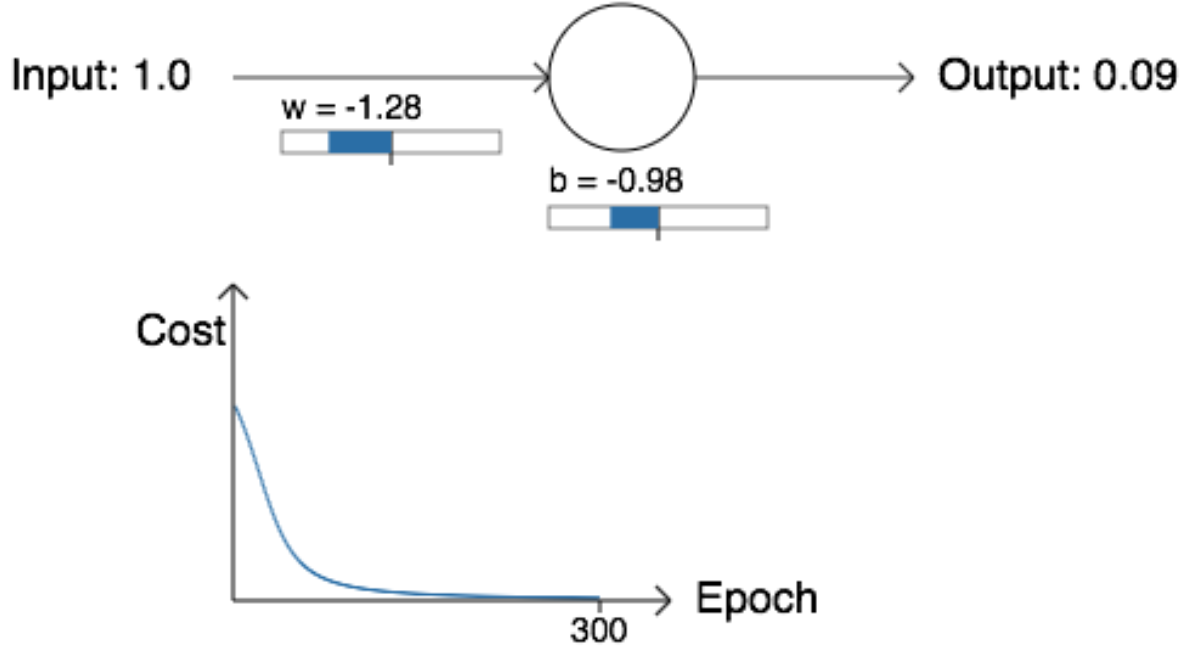
\includegraphics[scale=.4]{images/best_practices/first_graph.png}
    \centering
\end{figure}



Questo è il grafico della funzione costo quando i pesi sono inizializzati a $w=0.6$ e $b=0.9$. In questo caso si vede che facciamo piuttosto bene, in quanto si vede la funzione costo è quasi zero, il che significa che stiamo approssimando il risultato molto bene.



\begin{figure}[h]
    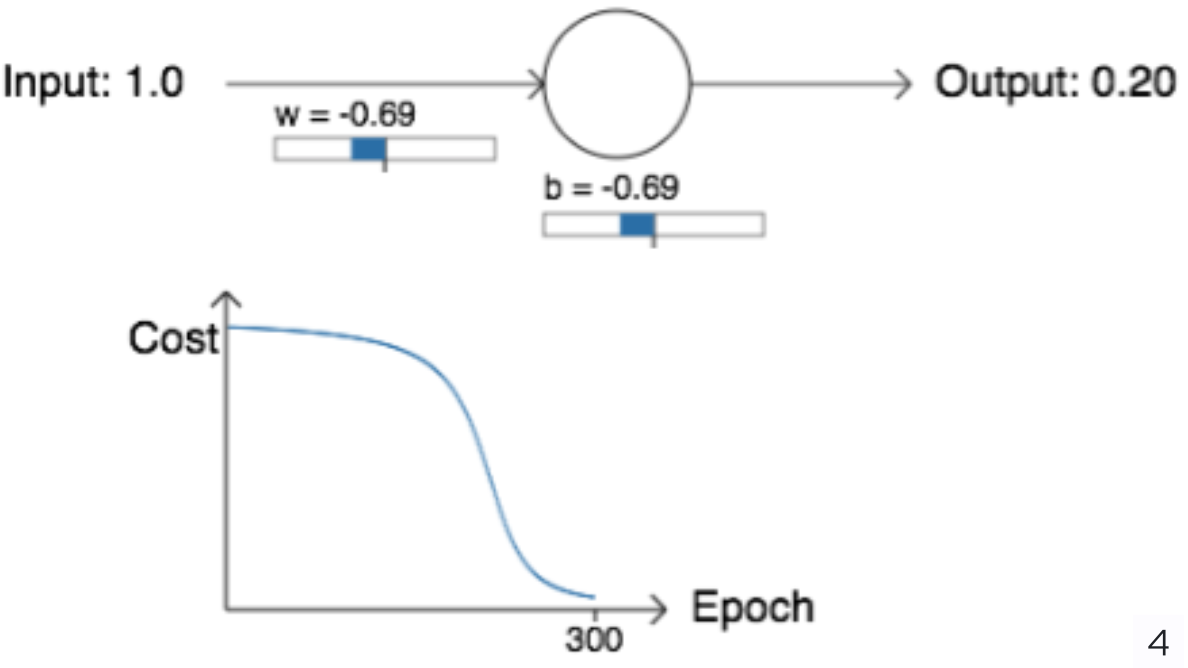
\includegraphics[scale=.4]{images/best_practices/second_graph.png}
    \centering
\end{figure}



Questo è il grafico della funzione costo quando i pesi sono inizializzati a $w=2.0$ e $b=2.0$. In questo caso si vede bene che passiamo i due terzi del tempo a non impararare praticamente niente (la curva è abbastanza costante).
\newline
\newline
Perchè accade questo? Ricordiamo che, per questo caso particolare, $C=\frac{(y-z)^2}{2}$ e $z=\sigma(a)=\sigma(wx+b)$. Tenendo questo in mente è facile vedere che:
\begin{equation}
    \frac{\partial C}{\partial w} = (y-z)\sigma'(a)x=z\sigma'(a)   
\end{equation}
e che
\begin{equation}
    \frac{\partial C}{\partial b} = (z-y)\sigma'(a)x=z\sigma'(z)   
\end{equation}
%ricontrollare queste formule, sono uguali
dove, in entrambe le formule, la seconda uguaglianza è ottenuta con le sostituzioni $x=1$ (input) e $y=0$ (output). La formula ci dice che la rete impara solo e soltanto se la derivata della funzione di schiacciamento, cioè $\sigma'$, non è piatta. Infatti, se ci troviamo in punti in cui la sigmoide è piatta, il fattore $z\sigma'(a)$ è quasi zero così come lo è anche la derivata. Questo è il motivo per cui non impareremmo niente.
\newpage
Il problema nel secondo esempio è tale che, scegliendo $w=2.0$ e $b=2.0$ come valori iniziali dei parametri della rete, iniziamo il learning in un punto in cui $z=2\times1+2=4$ e in quel punto la funzione sigmoide è molto piatta, quindi la sua derivata è quasi zero.
\begin{figure}[h]
    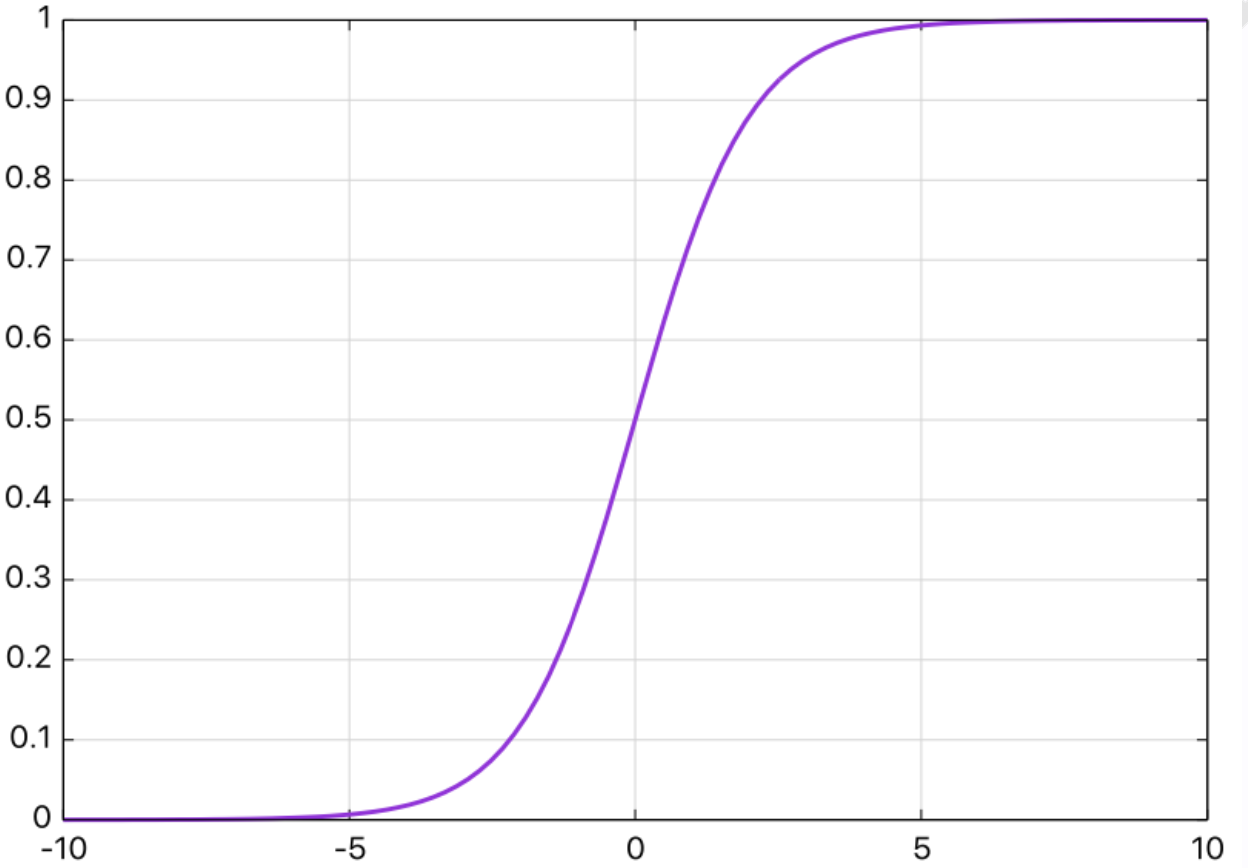
\includegraphics[scale=.4]{images/best_practices/slow_learn.png}
    \centering
\end{figure}

\subsection{La Cross-Entropy} La \textbf{cross-entropy cost function risolve il problema dello slow learning} senza cambiare la funzione di attivazione (cioè $\sigma$ rimane definita come la funzione sigmoide). 


La cross-entropy è definita come:
\begin{equation}
    C=-\frac{1}{n}\sum_x[y\ln{z}+(1-y)\ln{(1-z)}]
\end{equation}
dove, come sempre, $y$ è l'output desiderato e $z$ è l'attivazione del neurone.
\begin{figure}[h]
    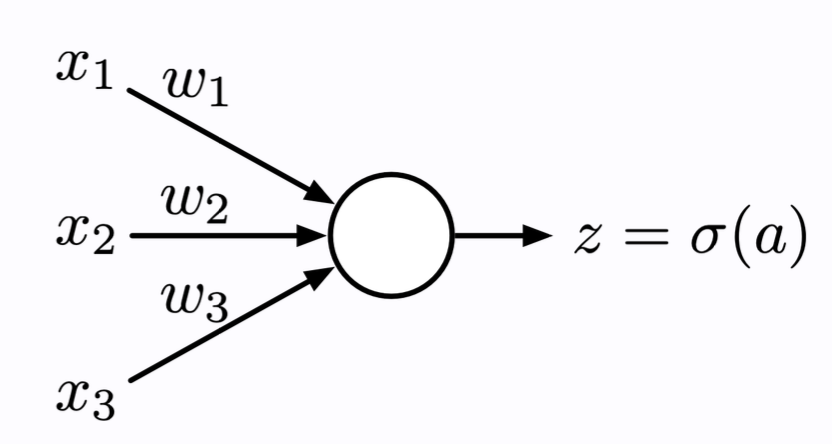
\includegraphics[scale=.5]{images/best_practices/cross_entropy.png}
    \centering
\end{figure}




\textbf{Nota}: come mostra l'immagine, stiamo sempre considerando una rete di un singolo neurone, ma nel caso leggermente più generale dove abbiamo più di un input: $a=\sum_jw_jx_j+b$.
\newline
\newline
Notiamo che $C$ si comporta ancora come una funzione costo:
\begin{itemize}
    \item se $y=1$ e $z\approx1$, allora:
        \begin{equation}
            -(y\ln{z}+(1-y)\ln{(1-z)})\approx0
        \end{equation}
    \item se $y=1$ e $z\approx0$, allora:
        \begin{equation}
            -(y\ln{z}+(1-y)\ln{(1-z)})\approx\infty.
        \end{equation}
\end{itemize}
La stessa cosa vale per $y=0$, $z\approx0$ e $y=0$, $z\approx1$.
Per finire: la \textbf{cross-entropy function} è sempre positiva e tende a zero come gli output calcolati tendono agli output desiderati.
\newline
\newline
\textbf{Cross Entropy}: $C=-\frac{1}{n}\sum_x[y\ln{z}+(1-y)\ln{(1-z)}]$, questa è un'espressione molto utile se usata come funzione costo, perchè ciò che noi vogliamo da una funzione costo è che essa sia grande quando sbagliamo e piccola quando invece stiamo facenod bene. In questo caso stiamo assumendo che il problema sia binario, quindi possiamo avere $y=0$ o $y=1$, $z\in[0,1]$ è l'output di una sigmoide. Vogliamo che $y$ e $z$ siano concordi. Nel caso in cui $y=1$ abbiamo che il secondo termine della somma, cioè $(1-y)\ln{(1-z)}$, sparisce e il secondo termine diventa semplicemente $\ln{z}$. Quest'ultimo vale $0$ se $z=1$, e quindi se $z$ e $y$ sono concordi, altrimenti (vedere grafico di $\ln$) diminuisce in maniera esponenziale. Lo stesso ragionamento si può fare se $y=0$. Sostanzialmente questo è il motivo per cui questa \textbf{è una buona funzione costo}. 


Mostriamo ora come perchè si combina bene con la sigmoide:
\begin{equation}
    \begin{array}{l}
    \frac{\partial C}{\partial w_j}=-\frac{1}{n}\sum_\text{x}\frac{y}{\sigma(a)}\frac{\partial \sigma}{\partial w_j}-\frac{1-y}{1-\sigma(a)}\frac{\partial \sigma}{\partial w_j}\\
    =-\frac{1}{n}\sum_\text{x}\Big( \frac{y}{\sigma(a)}-\frac{1-y}{1-\sigma(a)} \Big) \sigma'(a)x_j\\
    =-\frac{1}{n}\sum_\text{x}\Big( \frac{(1-\sigma(a))y-(1-y)\sigma(a)}{\sigma(a)(1-\sigma(a))}\Big) \sigma'(a)x_j\\
    =-\frac{1}{n}\sum_\text{x}\Big( \frac{y-y\sigma(a)-\sigma(a)+y\sigma(a)}{\sigma(a)(1-\sigma(a))}\Big) \sigma'(a)x_j\\
    =-\frac{1}{n}\sum_\text{x}\Big( \frac{y-\sigma(a)}{\sigma(a)(1-\sigma(a))}\Big) \sigma'(a)x_j\\
    =-\frac{1}{n}\sum_\text{x}\Big( \frac{y-\sigma(a)x_j}{\sigma(a)(1-\sigma(a))}\Big) (\sigma'(a)-y).
    \end{array}
\end{equation}

La derivata della sigmoide è:
\begin{equation}
    \sigma'(a)=\frac{d}{da}\Big(\frac{1}{1+e^{-a}} \Big)=
    \frac{e^{-a}}{(1+e^{-a})^2}=\sigma(a)(1-\sigma(a))
\end{equation}
come conseguenza si ha:
\begin{equation}
    \frac{\partial C}{\partial w_j}=\frac{1}{n}\sum_\text{x}x_j(\sigma(a)-y)
\end{equation}
la quale è una bellissima espressione perchè mostra che il tasso di apprendiamento dipende solo da quanto bene l'unità di output sta approssimando l'output desiderato. In altri termini, \textbf{mostra che maggiore è l'errore, maggiore è la velocità con cui l'unità apprenderà}.
\newline
\newline
Similmente, si può dimostrare:
\begin{equation}
    \frac{\partial C}{\partial b}=\frac{1}{n}\sum_\text{x}(\sigma(a)-y).
\end{equation}
\subsubsection{L'apprendimento tramite la Cross-Entropy}


\begin{figure}[!h]
    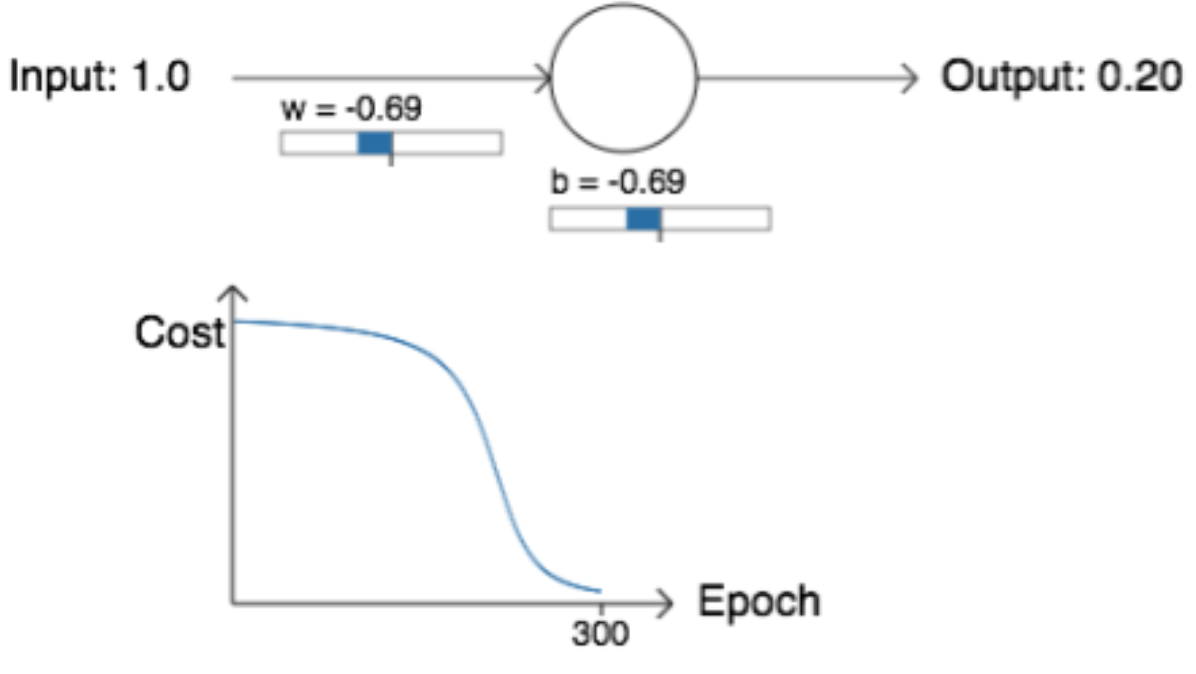
\includegraphics[scale=.4]{images/best_practices/first_graph_ce.png}
    \centering
\end{figure}



questo è il grafico della funzione costo \textbf{quadratica} quando i pesi sono inizializzati a $w=2.0$ e $b=2.0$.



\begin{figure}[h]
    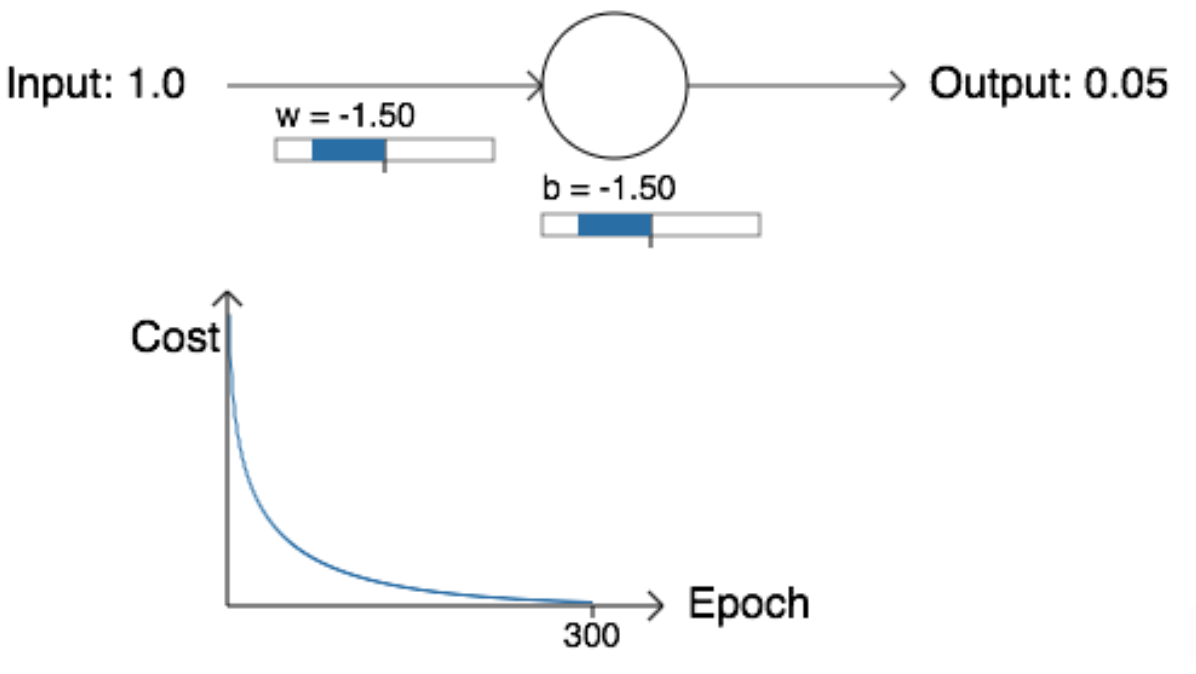
\includegraphics[scale=.4]{images/best_practices/second_graph_ce.png}
    \centering
\end{figure}


questo è il grafico della funzione costo \textbf{cross-entropy} quando i pesi sono inizializzati a $w=2.0$ e $b=2.0$.

Tutta la discussione fino a questo momento era concentrata su un singolo neurone. In ogni caso, è semplice generalizzare la cross-entropy ad una \textbf{many neuron, multy layer network}. Assumiamo che $y=y_1,y_t,\dots$ siano i valori desiderati dei neuroni output. Per questo caso più generale, la cross-entropy cost function è definita come segue:
\begin{equation}
    C=-\frac{1}{n}\sum_x\sum_j[y_j\ln{z_j^\text{l}}+(1-y_j)\ln{(1-z_j^\text{l})}].
\end{equation}

\subsection{Soft-Max + Log-Likelihood}
Fino ad ora abbiamo considerato architetture in cui le unità di output sono basate su funzioni di attivazioni sigmoidali e abbiamo dimostrato che, in questi casi, la cross-entropy è una cost function particolarmente vantaggiosa.


Un'altra architettura molto popolare che ha gli stessi benefici ed è particolarmente adatta quando il problema sottostante richiede la predizione di una distribuzione di probabilità, è basata sulla \textbf{soft-max activation unit}:
\begin{equation}
    z^\text{L}_j=\frac{e^{a^\text{L}_j}}{\sum_ke^{a^\text{L}_j}}
\end{equation}
e sulla \textbf{log-likelihood come funzione costo}:
\begin{equation}
    C\equiv -\ln{z}^\text{L}_y.
\end{equation}
Anche questa è una buona funzione costo perchè se il neurone che abbiamo selezionato ha un valore vicino ad uno (cioè è il neurone corrispondente alla classe corretta, se lo è dovrebbe avere un valore vicino ad uno) allora il logaritmo naturale di quel valore è quasi zero, il che significa che ha un costo bassissimo o non ha costo. Al contrario, se il valore è zero siamo molto penalizzati.


Tutti gli altri valori nell'output layer \textbf{non hanno peso in questo procedimento}, questo perchè abbiamo già una dipendenza da tutti gli altri neuroni, visto che tutti \textbf{partecipano nella soft-max}. 
\newline
\newline
\textbf{Nota}: c'è stato un leggero abuso di notazione rispetto ad $y$. In precedenza era infatti utilizzata per indicare \textbf{l'indice  dell'etichetta corretta}, ora è invece utilizzato per denotare \textbf{il vettore avente il componente corrispondente alla classificazione corretta settato ad 1 e a 0 tutti gli altri}.
\newpage
\paragraph{Soft-Max.}Come dovrebbe essere evidente, la soft-max activation function garantisce che:
\begin{itemize}
    \item ogni attivazione $z^\text{L}_j\in(0,1)$ (notare che gli estremi non sono inclusi, perchè guardando il grafico della funzione si vede che quei valori non sono mai toccati);
    \item $\sum_jz^\text{L}_j=1$.
\end{itemize}
Quindi il comportamento collettivo delle unità di output può essere interpretato come una previsione su una distribuzione di probabilità in cui $z^\text{L}_j=P(j|x)$ .

\paragraph{Log-Likelihood.} Anche se potrebbe non sembrare immediatamente evidente, la log-likelihood function si comporta esattamente come ci aspetteremmo da una funzione costo:
\begin{itemize}
    \item se la rete \textbf{calcola} l'output corretto, allora $z^\text{L}_y\approx1$ e $C=-\ln{z^\text{L}_y}\approx0$;
    \item se la rete \textbf{non calcola} l'outout corretto, allora $z^\text{L}_y\approx0$ e $C$ assumerà un valore grande.
\end{itemize}


\paragraph{Lo Slow Learning Problem.} Come menzionato prima, l'architettura soft-max + log-likelihood non soffre lo slow learning problema. Infatti, non è difficile dimostrare che:
\begin{itemize}
    \item $\frac{\partial C}{\partial w_{jk}^\text{L}}= z^{\text{L}-1}_k(z^{\text{L}}_j-y_j)$;
    \item $\frac{\partial C}{\partial w_j}=z^{\text{L}}_j-y_j$.
\end{itemize}
\newpage
\section{Inizializzazione dei parametri}
\textbf{L'inizializzazione dei parametri può avere un impatto significativo sulla performance di generalizzazione e sulla velocità di convergenza}. Sfortunatamente c'è poca teoria che suggerisca come inizializzare nella maniera più appropriata i parametri:



Molti approcci includono:
\begin{itemize}
    \item rottura della simmetria;
    \item mantenimento costante della varianza dei parametri.
\end{itemize}


\paragraph{Simmetry breaking.} Consideriamo una fully connected neural network. Se i parametri sono inizializzati in maniera uguale (una scelta comune potrebbe essere lo zero), tutti i neuroni calcoleranno la stessa funzione e tutti potrebbero essere aggiornati nello stesso modo. Per affrontare questo problema, un approccio comune è quello di \textbf{inizializzare i parametri in maniera randomica}, usando o una distribuzione uniforme nel range $[-\epsilon,+\epsilon]$ p una distribuzione Gaussiana $\mathcal{N}[0,\epsilon^2]$.

\paragraph{Keeping the variance constant.} Anche la scelta di $\epsilon$ è molto importante. Pesi troppo piccoli o troppo grandi potrebbero contriubuire ad avere un grandente molto grande o molto piccolo, il quale causerebbe o una \textbf{gradient explosion} o una \textbf{gradient implosion}. 


Sono stati fatti molti tentativi per trovare una buona inizializzazione dei parametri. Per esempio:
\begin{itemize}
    \item per la \textbf{ReLu} activation unit la \textit{He initialization} dovrebbe rendere il grandiente approssimativamente uguale ad $1$:
    \begin{equation}
        \epsilon=\sqrt{\frac{2}{M}}
    \end{equation}
    dove $M$ è il numero di input del neurone che deve essere inizializzato.
\end{itemize}

\paragraph{He initialization.} Assumiamo che ogni layer $l$ della rete valuta:
\begin{equation}
    a^l_i \sum^M_{j=1}w_{ij}z_j^{l-1},
\end{equation}
\begin{equation}
    z^l_i=\text{ReLU}(a_i^l).
\end{equation}
Assumiamo che i pesi siano inizializzati attingendo da una Gaussiana $\mathcal{N}[0,\epsilon^2]$ e assumiamo che gli output del layer $l-1$ abbiamo media $0$ e varianza $\lambda^2$. \textbf{Si può dimostrare che}:
\begin{equation}
    \text{var}[z^l_j]=\frac{M}{2}\epsilon^2\lambda^2.
\end{equation}
L'idea principale nella He initialization è il \textbf{mantenimento costante della varianza tra i layer}, il che implica che:
\begin{equation}
    \epsilon=\frac{2}{M}.
\end{equation}

\paragraph{Xavier (a.k.a. Glorot) initialization.} La \textbf{Xavier initialization}, ispirata dal lavoro di Xavier Glorot, è pensata per funzioni di attivazione simmetriche attorno alllo $0$ (come \textbf{la sigmoide} e \textbf{la tangente iperbolica}). Essa campiona le inizializzazioni dei pesi da una distribuzione uniforme $U[-\epsilon,\epsilon]$:
\begin{itemize}
    \item inizializzazione di Xavier: $\epsilon:\frac{1}{\sqrt{M}}$,
    \item inizializzazione di Xavier normalizzata: $\epsilon = \frac{6}{\sqrt{N+M}}$.
\end{itemize}
Dove $M$ è il numero di input del neurone e $N$ è il numero di unità nel layer.
\newpage
\section{Convergenza}
Molti fatti interessanti si possono dimostrare  riguardanti la convergenza del metodo della discesa del gradient:
\begin{enumerate}
    \item i componenti di \textbf{w evolvono indipendentemente};
    \item la discesa del gradiente conduce a una \textbf{convergenza lineare} nell'intorno di un minimo;
    \item il \textbf{tasso di convergenza} è governato da $1-\Big( \frac{2\lambda_{\text{min}}}{\lambda_{\text{max}}} \Big)$.
\end{enumerate}
\textbf{**NOTA**: da questo punto il prof salta fino alle proprietà a pagina 61 (\textit{in sintesi...})}.
\newline
\newline
Consideriamo ora l'approssimazione quadratica della funzione di errore attorno ad un punto \textbf{w}$^*$ il quale rappresenta un minimo della funzione:
\begin{equation}
    E(\textbf{w})=E(\textbf{w}^*)+\nabla E(\textbf{w}^*)^T(\textbf{w}-\textbf{w}^*)+\frac{1}{2}(\textbf{w}-\textbf{w}^*)^T\textbf{H}(\textbf{w}-\textbf{w}^*).
\end{equation}
In questo caso non ci sono termini lineari perchè $\nabla E=0$ in \textbf{w}$^*$, portando a:
\begin{equation}
    E(\textbf{w})=E(\textbf{w}^*)+\frac{1}{2}(\textbf{w}-\textbf{w}^*)^T\textbf{H}(\textbf{w}-\textbf{w}^*).
\end{equation}

Consideriamo ora l'(equazione di autovalori? = eingevalue equation) per l'Hessiana:
\begin{equation}
    \textbf{Hu}_i=\lambda_i\textbf{u}_i
\end{equation}
dove ${\textbf{u}_i}_i$ sono gli autovettori di \textbf{H} e formano una base ortonormale:
\begin{equation}
    \forall i : ||\textbf{u}_i||=1 \land \forall i,j:\textbf{u}_i^T\textbf{u}_j=\delta_{ij},
\end{equation}
dove
\begin{equation}
    \delta_{ij}=I_{i=j}=f(x)= 
    \begin{cases}
        1,& \text{se } i=j\\
        0,              & \text{altrimenti}
    \end{cases}
\end{equation}
Siccome ${\textbf{u}_{i}}_i$ è una base ortonormale, possiamo riscrivere qualsiasi vettore in termini di una combinazione lineare dei vettori $\textbf{u}_i$, che ci portano a scrivere:
\begin{equation}
    \textbf{w}-\textbf{w}^*=\sum_i\alpha_i\textbf{u}_i.
\end{equation}
Detto questo possiamo dimostrare che:
\begin{equation}
    E(\textbf{w})=E(\textbf{w}^*)+\frac{1}{2}\sum_i\lambda_i\alpha^2_i.
\end{equation}
\textbf{Dimostrazione:}
\begin{equation}
\begin{split}
  E(\textbf{w})=E(\textbf{w}^*)+\frac{1}{2}(\textbf{w}-\textbf{w}^*)^T\textbf{H}(\textbf{w}-\textbf{w}^*)\\
  =E(\textbf{w}^*)+\frac{1}{2}\Big(\sum_i\alpha_i\textbf{u}_i\Big)^T \textbf{H}\Big(\sum_i\alpha_i\textbf{u}_i \Big)^T\\
  =E(\textbf{w}^*)+\frac{1}{2}\Big(\sum_i\alpha_i\textbf{u}_i \Big)^T \Big(\sum_i\alpha_i\textbf{H} \textbf{u}_i \Big)^T\\
   =E(\textbf{w}^*)+\frac{1}{2}\Big(\sum_i\alpha_i\textbf{u}_i \Big)^T \Big(\sum_i\alpha_i\lambda_i \textbf{u}_i \Big)^T\\
   =E(\textbf{w}^*)+\frac{1}{2}\sum_i\lambda_i\alpha^2_i
\end{split}
\end{equation}
\newpage
Ciò implica che $\nabla E=\sum_i\alpha_i\lambda_i\textbf{u}_i$.



\textbf{Dimostrazione:}
\begin{equation}
\begin{split}
    \nabla E(\textbf{w})=\nabla\Big( E(\textbf{w}^*)+\frac{1}{2}\sum_i\lambda_i\alpha_i^2 \Big)\\
    =\frac{1}{2}\sum_i\lambda_i2\alpha_i\nabla\alpha_i.
\end{split}
\end{equation}

Ora calcoliamo $\nabla\alpha_i$, partendo dal richiamare che $\textbf{w}-\textbf{w}^*=\sum_j\alpha_j\textbf{u}_j$, da qua:
\begin{equation}
    \begin{split}
        \textbf{u}_i^T(\textbf{w}-\textbf{w}^*)=\textbf{u}^T_i\Big( \sum_j\alpha_j\textbf{u}_j \Big)\\
        \textbf{u}_i^T(\textbf{w}-\textbf{w}^*)=\alpha_i\\
        \sum_jw_j\textbf{u}_{ij}-\sum_jw^*_j\textbf{u}_{ij}=\alpha_i\\
        \frac{\partial}{\partial w_k}\Big( \sum_jw_j\textbf{u}_{ij}-\sum_jw^*_j\textbf{u}_{ij} \Big)=\textbf{u}_{ik} =  \frac{\partial \alpha_i}{\partial w_k} \Rightarrow \nabla_i=\textbf{u}_i.
    \end{split}
\end{equation}
In sintesi, abbiamo:
\begin{itemize}
    \item $\textbf{w}-\textbf{w}^*=\sum_i\alpha_i\textbf{u}_i\Rightarrow \Delta\textbf{w}=\sum_i\Delta\alpha_i\textbf{u}_i$;
    \item $\nabla E=\sum_i\alpha_i\lambda_i\textbf{u}_i$;
    \item $\Delta\textbf{w}=-\eta\nabla E$.
\end{itemize}
Queste relazioni ci portano a concludere che:
\begin{equation}
    \Delta a_i=-\eta\lambda_i\alpha_i\Rightarrow\alpha^{\text{new}}_i=(1-\eta\lambda_i)\alpha^{\text{old}}_i.
\end{equation}
\textbf{Dimostrazione:}
\begin{equation}
\begin{split}
    \Delta \textbf{w}=\sum_i\Delta\alpha_i\textbf{u}_i\Rightarrow-\eta\nabla E =\sum_i\Delta\alpha_i\textbf{u}_i\Rightarrow-\eta\sum_i\alpha_i\lambda_i\textbf{u}_i=\sum_i\Delta\alpha_i\textbf{u}_i \\
    \Rightarrow\sum_i\Delta\alpha_i\textbf{u}_i =\sum_i-\eta\lambda_i\alpha_i\textbf{u}_i
\end{split}
\end{equation}
Da $\textbf{u}^T_i(\textbf{w}-\textbf{w}^*)=\alpha_i$ segue che possiamo interpretare $\alpha_i$ come la \textbf{la distanza dal minimo lungo la direzione $\textbf{u}_i$}.


Inoltre, da $\alpha^{\text{new}}_i=(1-\eta\lambda_i)\alpha^{\text{old}}_i$, sappiamo che queste \textbf{distanze evolvono indipendetemente} e ad ogni step si riducono di una quantità proporzionale a $(1-\eta\lambda_i)$. Dopo $T$ step, abbiamo:
\begin{equation}
    \alpha^{(T)}_i=(1-\eta\lambda_i)^T\alpha^{(0)}_i.
\end{equation}
A condizione che $|1-\eta\lambda_i|<1$, il limite per $T\rightarrow\infty$ porta a $\alpha_i=0$, il che implica che abbiamo raggiunto il minimo della funzione errore.
\newpage
\textbf{L'ordine della convergenza è lineare} con tasso $1-\eta\lambda_i$ siccome:
\begin{equation}
    \lim_{T\rightarrow\infty}{\frac{\alpha^{(T)}_i-0}{(\alpha^{T-1}_i-0)^1}}=1-\eta\lambda_i.
\end{equation}
\begin{figure}[h]
    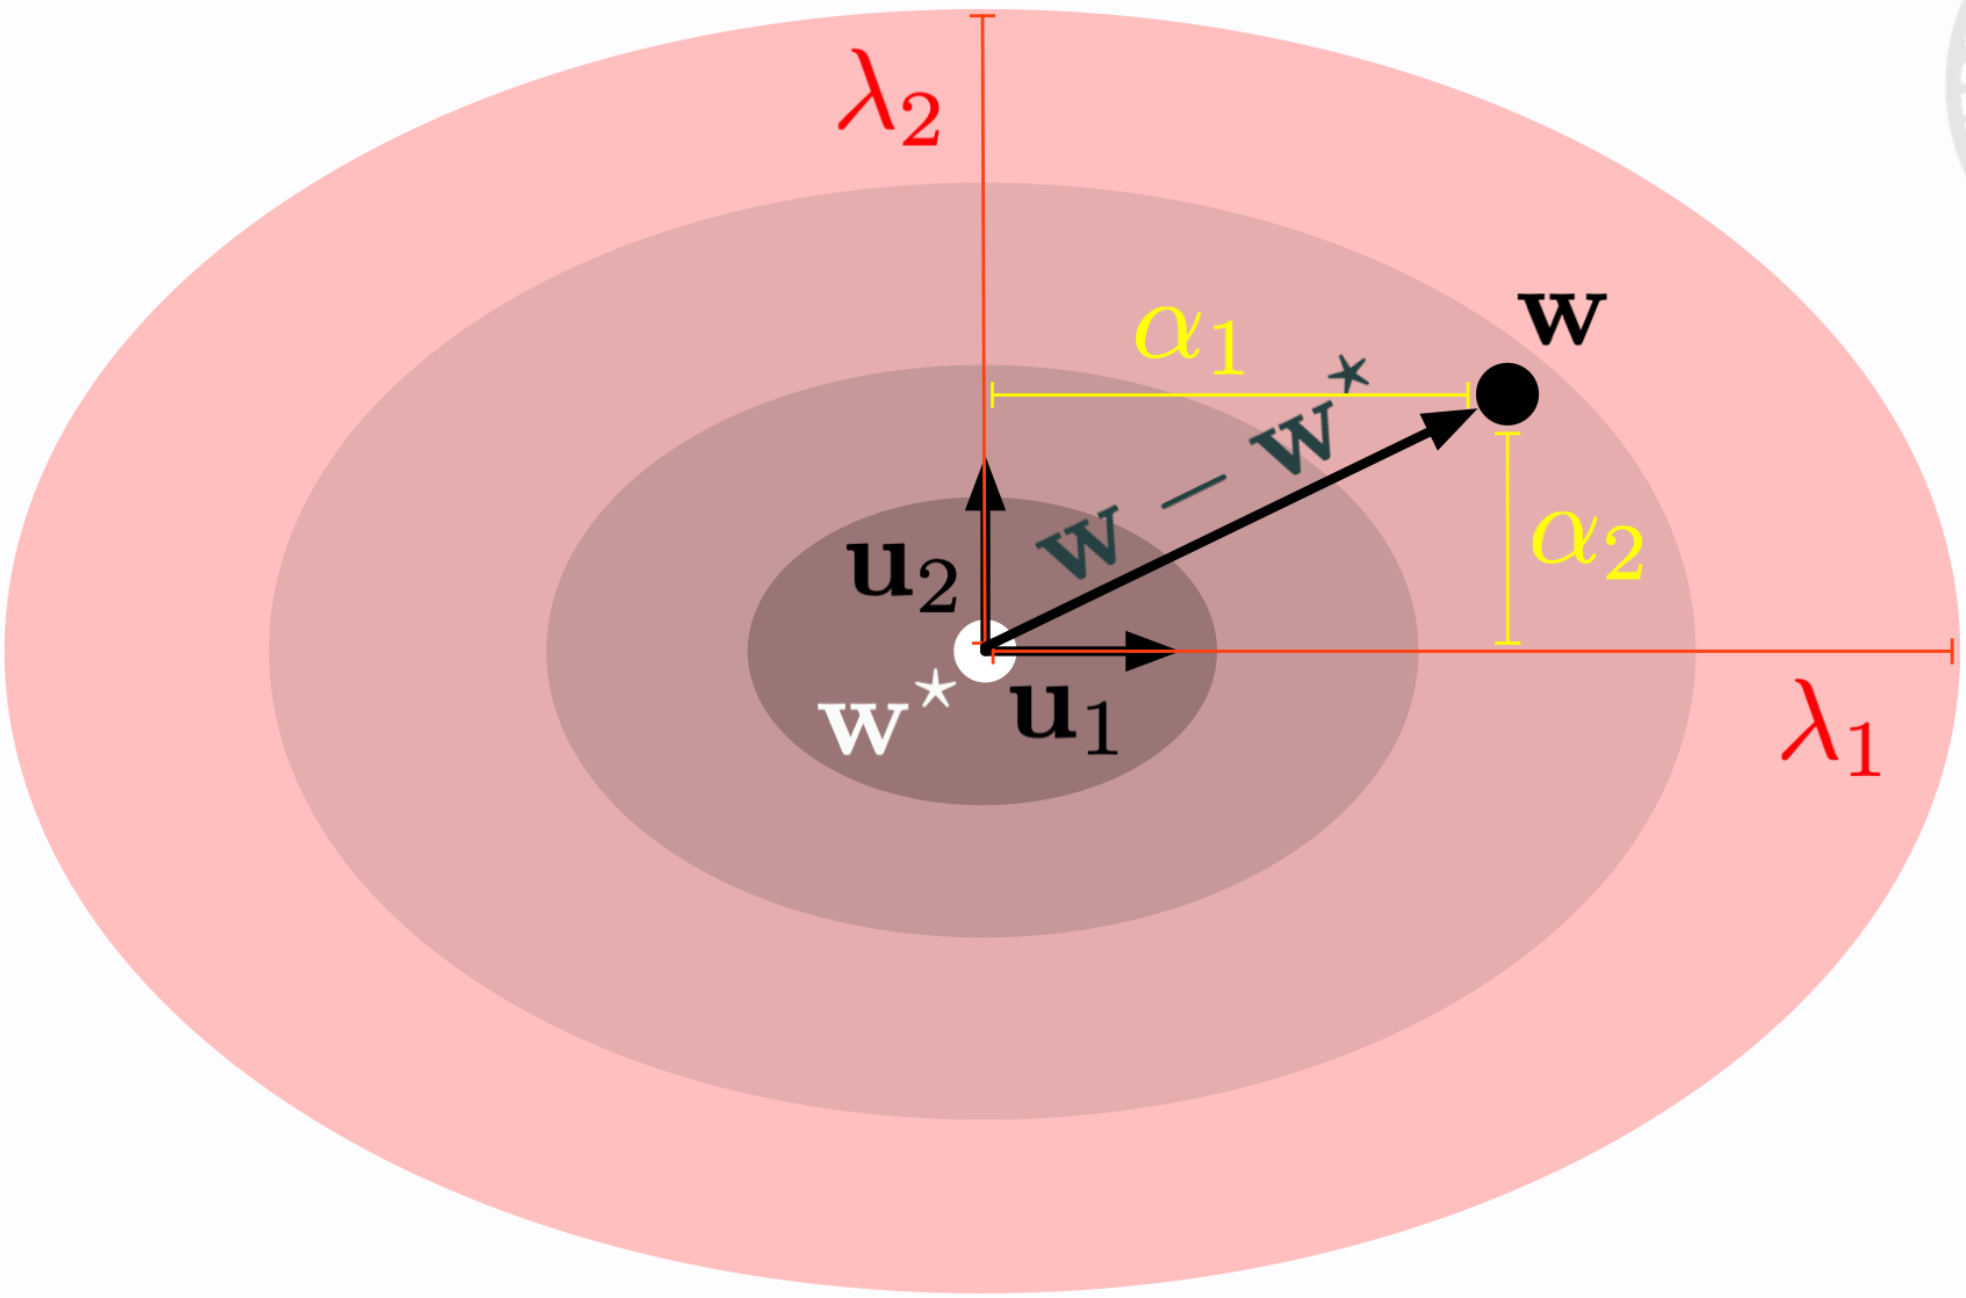
\includegraphics[scale=.3]{images/best_practices/convergence.png}
    \centering
\end{figure}


Decrementando $\eta$ possiamo migliorare la velocità di convergenza, ma dobbiamo assicurarci che $|1-\eta\lambda_i|<1$, che implica che \textbf{per garantire la convergenza} dobbiamo settare $\eta<\frac{2}{\lambda_{\text{max}}}$. 


\textbf{La convergenza più veloce} si ottiene quando $\eta=\frac{1}{\lambda_{\text{max}}}$. In questo caso il tasso di convergenza nella direzione di $\lambda_{\text{max}}$ è $0$, il quale implica che raggiungeremo il minimo con un singolo step.


Assumendo che $\eta=\frac{1}{\lambda_{\text{max}}}$, la direzione nella quale convergiamo in maniera più lenta in assoluto è data da $\lambda_{\text{min}}$. In questo caso il tasso di convergenza è
$1-\frac{\lambda_{\text{min}}}{\lambda_{\text{max}}}$.


Ciò implica che il caso peggiore si ha quando $\lambda_{\text{min}}$ è piccolo rispetto a $\lambda_{\text{max}}$, nel qual caso il tasso di convergenza è approssimativamente $1$ e la convergenza sarà molto lenta.



Il \textbf{reciproco} di $\frac{\lambda_{\text{min}}}{\lambda_{\text{max}}}$ è il \textbf{numero di condizionamento} della matrice Hessiana. Più grande è il numero di condizionamento, più lenta sarà la convergenza della discesa del gradiente.
\newline
\newline
Notiamo che quando $\lambda_{\text{min}}\ll\lambda_{\text{max}}$, la funzione errore avrà una forma molto allungata, la quale renderà la convergenza molto lonta a causa del fatto che il gradiente sarà molto piccolo nella direzione di $\lambda_{\text{min}}$.
\begin{figure}[h]
    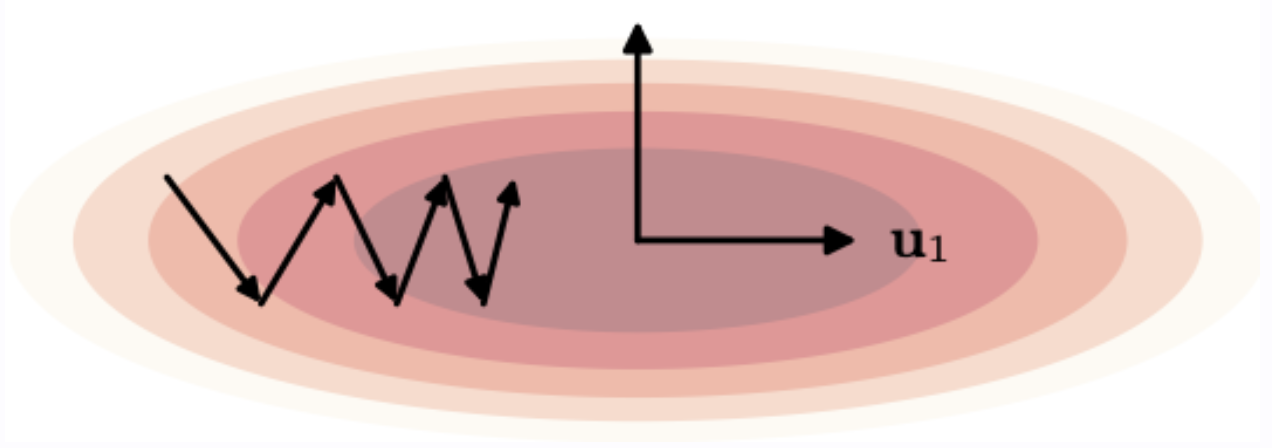
\includegraphics[scale=.5]{images/best_practices/shape.png}
    \centering
\end{figure}
\newpage
\section{Momentum e Learning Rate Scheduling}
Quando la convergenza è lenta, potrebbe essere utile aggiunere un \textbf{momentum term} alla formula della discesa del gardiente. Ciò aggiunge inerzia al movimento e attenua le oscillazioni mostrate di seguito.
\begin{figure}[h]
    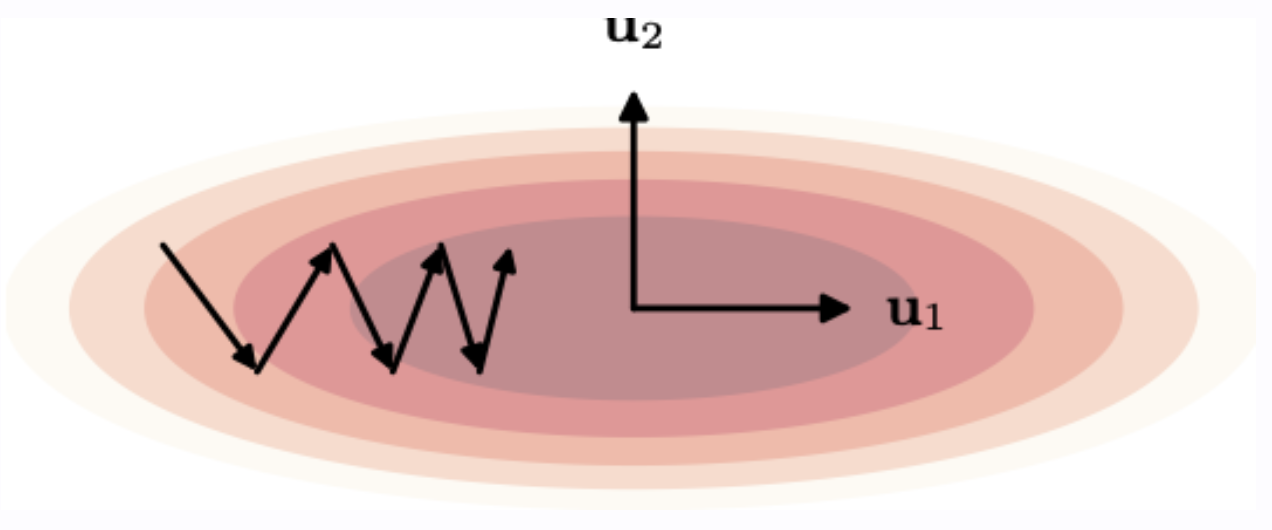
\includegraphics[scale=.5]{images/best_practices/momentum.png}
    \centering
\end{figure}


Ricordiamo ora la formula per l'aggiormaneto dei pesi nella rete:
\begin{equation}
    \textbf{w}^{(\tau)}=\textbf{w}^{(\tau-1)}+\Delta\textbf{w}^{(\tau-1)}.
\end{equation}
Quando aggiungiamo il momentum, il termine $\Delta\textbf{w}^{(\tau-1)}$ diventa:
\begin{equation}
    \Delta\textbf{w}^{(\tau-1)}=-\eta\nabla E(\textbf{w}^{(\tau-1)})+\mu\Delta\textbf{w}^{(\tau-2)},
\end{equation}
dove $\mu$ è il \textbf{momentum parameter}.
\newline
\newline
\textbf{In una regione di bassa curvatura}, se assumiamo che il gradiente e il momentum non cambiano, dopo una lunga serie di aggiornamenti avremo:
\begin{equation}
    \Delta\textbf{w}=-\eta\nabla E + \mu [-\eta\nabla E + \mu[ -\eta\nabla E + \dots] ] = -\eta\nabla E\{ 1+\mu+\mu^2+\dots \}=-\frac{\eta}{1-\mu}\nabla E,
\end{equation}
che, a condizione che $\mu<1$, implica che \textbf{il momentum sta facendo crescere il learning rate di un fattore pari a} $\frac{1}{1-\mu}$.



\textbf{In una regione di alta curvatura}, dove la discesa del gradiente è oscillatoria, \textbf{successivi contributi del momentum tendono ad annullarsi e l'effettivo learning rate sarà vicino a} $\eta$.



\textbf{Un valore tipico} per il parametro del momentum è $0.9$.

\paragraph{Learning rate scheduling.} E' vantaggioso cambiare il learning rate $\eta$ durante l'apprendimento. In pratica, i risultati migliori si ottengono usando un valore grande per $\eta$ all'inizio del training e riduncendo il learning rate nel tempo:
\begin{equation}
     \textbf{w}^{(\tau)}=\textbf{w}^{(\tau-1)}-\eta^{(\tau-1)}\nabla E(\textbf{w}^{(\tau-1)}).
\end{equation}
Esempi di learning schedules:
\begin{itemize}
    \item \textbf{lineare:} $\eta^{(\tau)}=(1-\frac{\tau}{K})\eta_0+(\frac{\tau}{K})\eta_K$, dove $\eta_0, \eta_K,K$ sono tre parametri e la formula è applicata fino a $K$ step. Dopo questi $K$ step, $\eta$ rimane fissato a $\eta_K$;
    \item \textbf{power law:} $\eta^{(\tau)}=\eta_0(1+\frac{\tau}{s})^c$;
    \item \textbf{decadimento esponenziale:} $\eta^{(\tau)}=\eta_0c^{\frac{\tau}{s}}$.
\end{itemize}
\newpage
\subsection{Ulteriori algoritmi}
Ulteriori perfezionamenti possono essere ottenuti notando che il cambiamento nel learning rate può essere ottimizzato separatamente per ogni direzione nello spazio dei parametri, cioè per ogni $w_{ij}$. I tre metodi di scheluding più popolari basati su questa idea sono:
\begin{itemize}
    \item \textbf{AdaGrad} (abbreviazione per \textit{Adaptive Gradient}): riduce ogni parametro di learning nel tempo utilizzando la somma accumulata dei quadrati di tutte le derivate calcolate per quei parametri. L'idea è di \textbf{ridurre il learning rate per quei parametri che hanno ricevuto grandi aggiornamenti nel passato};
    \item \textbf{RMSProp} (abbreviazione per \textit{Root Mean Square Propagation}): sostituisce la somma del quadrato dei gradienti di AdaGrad con con una media ponderata esponenzialmente. Risolve il problema di AdaGrad per cui gli aggiornamenti dei pesi tendono a diventare troppo piccoli;
    \item \textbf{AdaM} (abbreviazione per \textit{Adaptive Moments}): combina RMSProp con il momentum. Probabilmente è il metodo di ottimazione più utilizzato nel deep learning.
\end{itemize} 
\newpage
\section{Normalizzazione}
Gestire valori che variano in intervalli molto diversi e dover affrontare gradienti \textbf{che svaniscono (vanishing)} o \textbf{che esplodono (exploding)} sono i problemi principali del deep learning.


La normalizzazione dei pesi prova a gestire questi problemi, mantenendo i valori calcolati dalla rete in un range ragionevole. 


Abbiamo tre approcci principali:
\begin{itemize}
    \item data normalization;
    \item batch normalization;
    \item layer normalization.
\end{itemize}

\subsection{Data normalization} Se il set di dati ha variabili in input che includono range molto diversi, allora il cambiamento in una dimensione produrrà un cambiamento molto grande nell'output rispetto al cambiamento in un'altra dimensione.
\begin{figure}[h]
    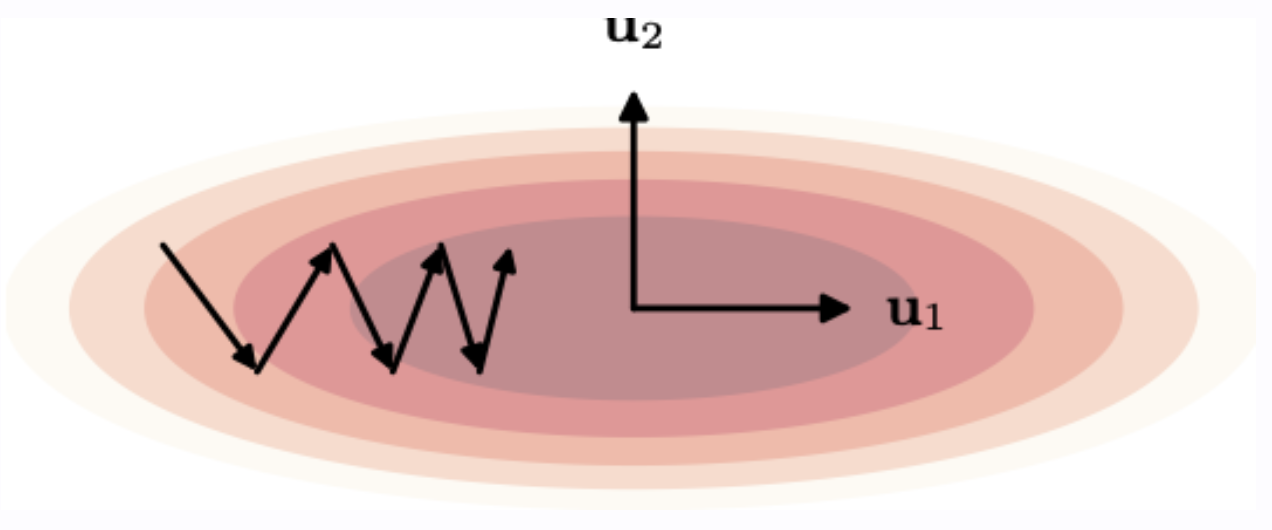
\includegraphics[scale=.25]{images/best_practices/momentum.png}
    \centering
\end{figure}



Per affrontare questo problema, come prima cosa calcoliamo media e varianza per ogni dimensione $i$:
\begin{equation}
    \mu_i=\frac{1}{N}\sum^N_{n=1}x_{ni},
\end{equation}
\begin{equation}
    \sigma^2_i=\frac{1}{N}\sum^N_{n=1}(x_{ni}-\mu_i)^2;
\end{equation}
poi riscaliamo tutti i data point utilizzando:
\begin{equation}
    \tilde{x}_{ni}=\frac{x_{ni}-\mu_i}{\sigma_i}.
\end{equation}
L'effetto di questa pratica è che la distribuzione degli esempi si comporterà approssimativamente come una Gaussiana con media $0$ e varianza $1$, la quale è una buona scelta per l'apprendimento.
\begin{figure}[h]
    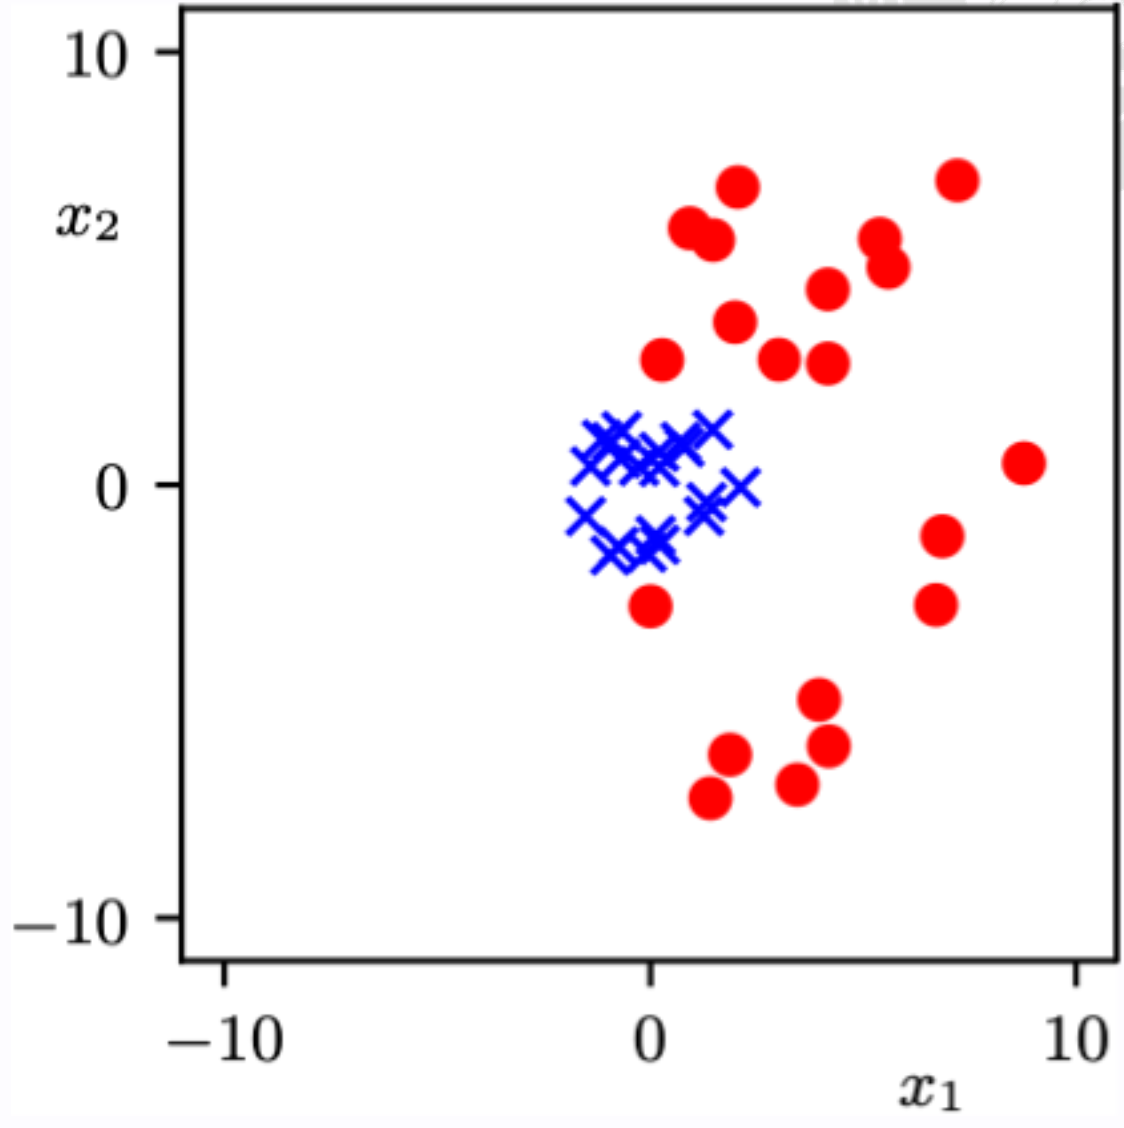
\includegraphics[scale=.25]{images/best_practices/data_norm.png}
    \centering
\end{figure}
\newpage
\subsection{Batch normalization}
Lo stesso ragionamento può essere applicato alle variabili (i pesi) di ogni hidden layer. 



Il fatto è che abbiamo risolto il problema per i dati in input ma essi vengono continuamente trasformati durante il loro spostamento all'interno della rete; a causa dei pesi nella rete possiamo ritrovarci in una situazione in cui l'output $z_i$ di un certo livello, il quale è input del livello successivo, torna ad avere una distribuzione sfasata, con alcune feature molto grandi e altre molto piccole. In questo contesto ci ritroviamo ad avere esattamente gli stessi problemi precedenti, rigurdanti il gradiente. Diventa quindi utile \textbf{rinormalizzare i dati dopo ogni layer}.



Sfortunatamente, \textbf{la normalizzazione per quei valori non può essere fatta una volta e valere per tutti}, tutti i calcoli devono essere fatti ogni volta che le variabili vengono aggiornate.


Uno dei modi per compiere questa normalizzazione è la \textbf{batch normalization}. La \textbf{batch normalization} invece di calcolare  la media e la varianza di tutti gli esempi, calcola solo quelle degli esempi del mini-batch. La differenza è che prima agivo su $x_i$, cioè l'input, ora agisco su $a_i$ che è il valore di pre attivazione del neurone. Quindi calcolo tutti gli $a_i$ e media e varianza su di essi. Dopo ciò normalizzo. 
\begin{figure}[h]
    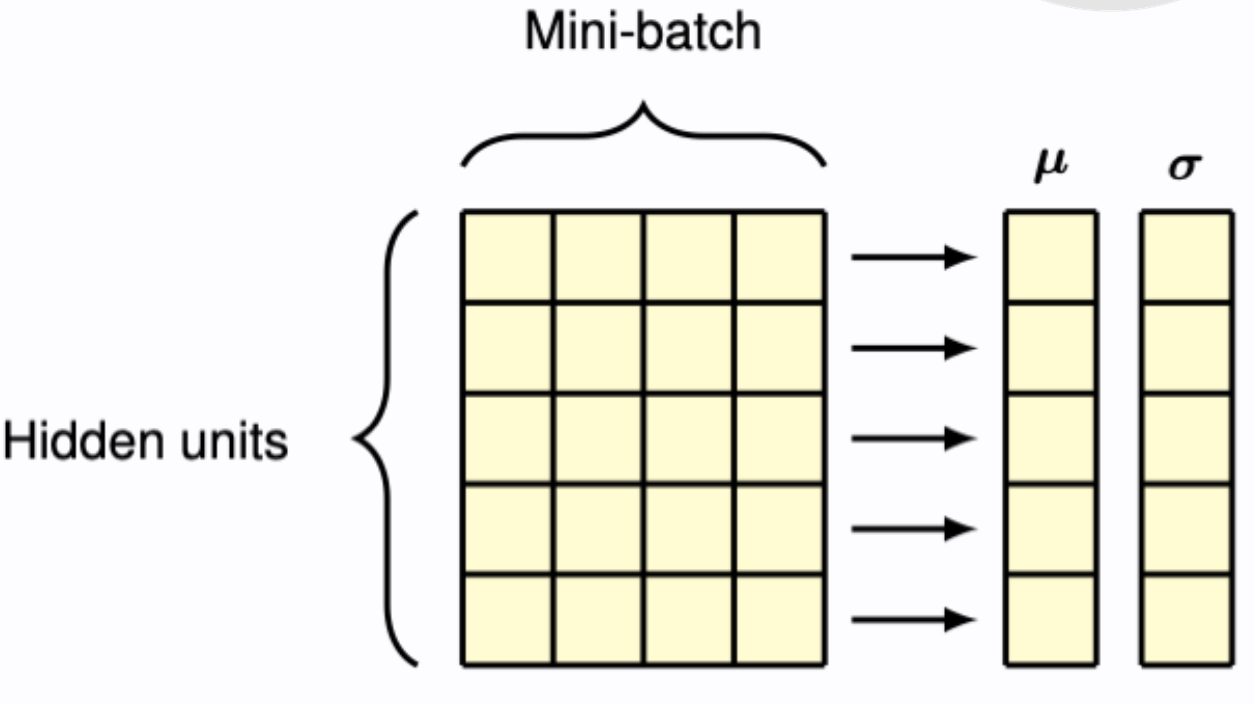
\includegraphics[scale=.3]{images/best_practices/batch_norm.png}
    \centering
\end{figure}



Consideriamo una unità hidden $z_i=h(a_i)$. Le quantità interessanti sono i valori di pre attivazione $a_i$ e i valori di post attivazione $z_i$. E' possibile normalizzzare i valori pre o post attivazione, entrambi gli approcci funzionano bene nella pratica.



Per esempio, per normalizzare i valori di pre attivazione, bisognerebbe calcolare:
\begin{equation}
    \mu_i =\frac{1}{K}\sum^K_{n=1}a_{ni},
\end{equation}
\begin{equation}
    \sigma^2_i =\frac{1}{K}\sum^K_{n=1}(a_{ni}-\mu_i)^2,
\end{equation}
\begin{equation}
    \hat{a}_{ni}=\frac{a_{ni}-\mu_i}{\sqrt{\sigma^2_i+\delta}},
\end{equation}
dove $K$ è la dimensione del mini batch e $\delta$ evita problemi numerici quando $\sigma^2_i$ è piccolo.


Uno dei problemi infatti sta nel fatto che, lavorando con i mini-batch, potrei ritrovarmi ad avere pochi esempi e quindi calcolare una varianza poco accurata (in particolare avere valore molto piccolo può causare problemi numerici, visto che la deviazione standard si trova a denominatore).



Questo tipo di normalizzazione riduce inoltre la capacità rappresentativa delle hidden units. Per compensare questo fatto, si possono \textbf{riscalare i valori di pre attivazione} in modo che abbiano media $\beta_i$ e deviazione standard $\lambda_i$:
\begin{equation}
    \tilde{a}_{ni}=\lambda_i\hat{a}_{ni}+\beta_i.
\end{equation}
Mentre all'inizio la media e la varianza attraverso un minibatch erano calcolate da una complessa funzione di pesi e bias, ora sono determinati da due semplici parametri indipendenti, i quali risultano essere molto più semplici da apprendere dalla discesa del gradiente.



Una volta che il training è completato, non avremo più minibatch per calcolare la normalizzazione dei fattori. Per far fronte a ciò, manteniamo una media mobile di media e varianza all'interno del modello, usata in \textbf{inference time} per riscalare i valori:
\begin{equation}
    \bar{\mu}^{(\tau)}_i=\alpha\bar{\mu}^{(\tau-1)}_i+(1-\alpha)\mu_i,
\end{equation}
\begin{equation}
    \bar{\sigma}^{(\tau)}_i=\alpha\bar{\sigma}^{(\tau-1)}_i+(1-\alpha)\sigma_i,
\end{equation}
dove $0\leq\alpha\leq1$.
\newline
\newline
La \textbf{batch normalization} risulta essere molto efficace nella pratica, ma non risulta completamente comprensibile il perchè. Originariamente ciò è stato motivato come un modo per contrastare il problema del \textbf{internal covariate shift}: esso si presenta quando l'aggiornamento dei pesi negli strati precedenti della rete cambia la distribuzione dei valori visti dai layer successivi.


Studi successivi hanno mostrato che il covariate shift non è un fattore significante e che i miglioramenti derivano dallo \textbf{smoothing the error function landscape}.


\subsection{Layer normalization}
Invece di normalizzare gli esempi all'interno di un mini-batch per ciascuna hidden unit separatamente, la \textbf{layer normalization normalizza i valori delle hidden unit per ciascun data point separatamente}.
\begin{figure}[h]
    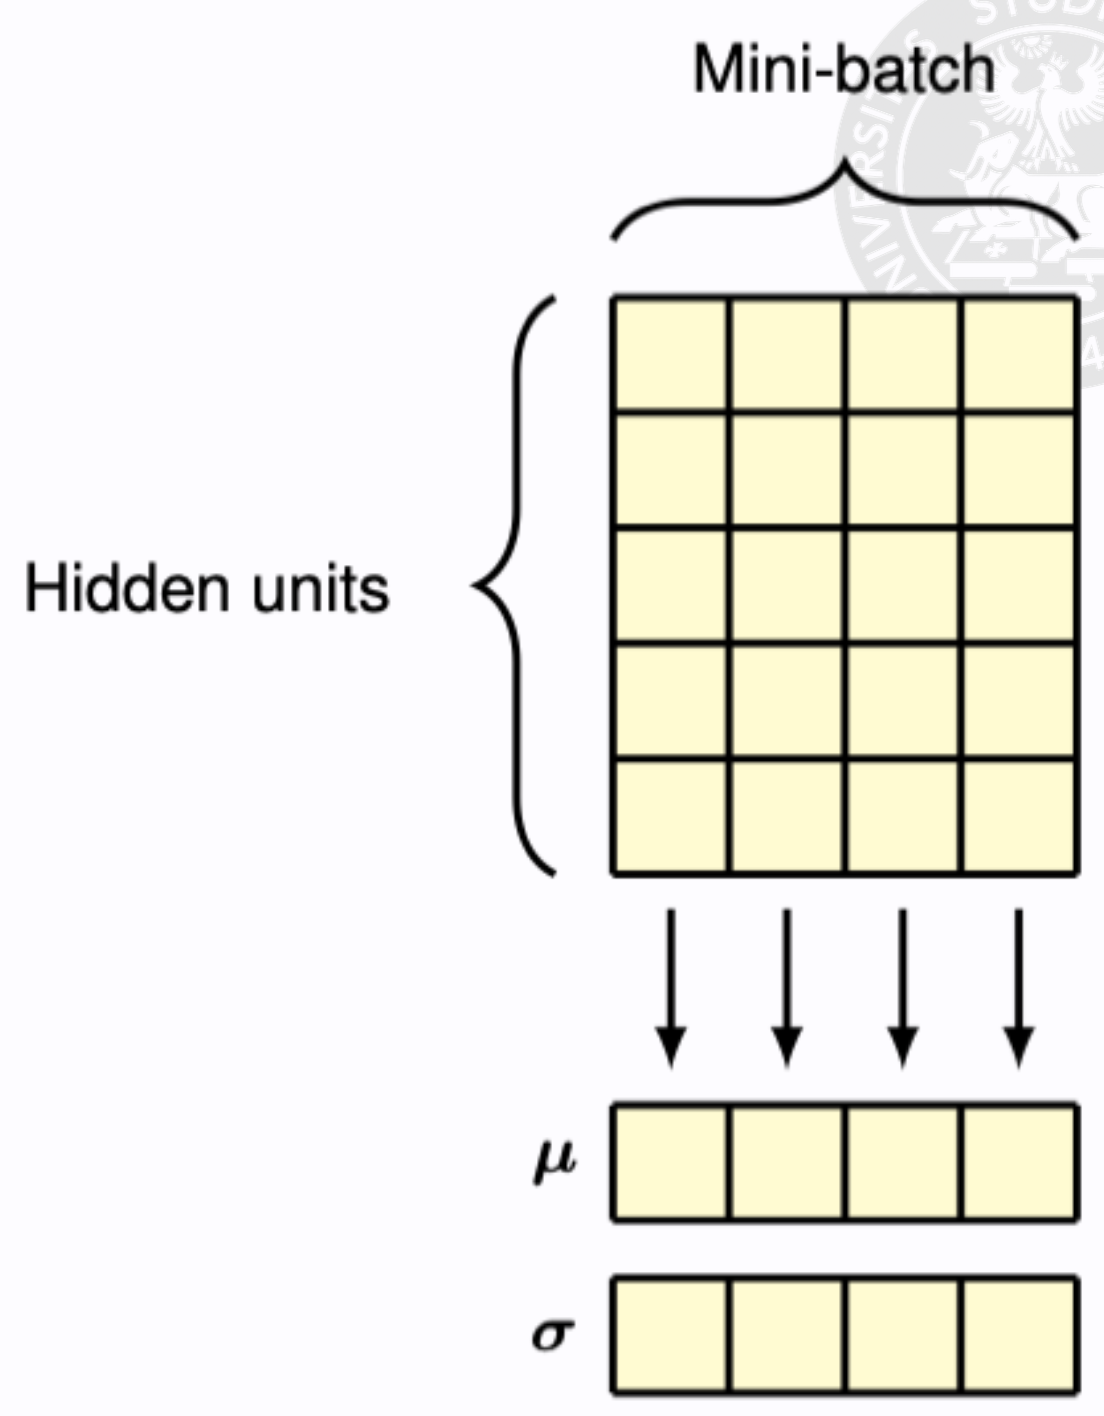
\includegraphics[scale=.4]{images/best_practices/layer_norm.png}
    \centering
\end{figure}


La \textbf{layer normalization} aggiorna i valori di pre attivazione come segue:
\begin{equation}
    \mu_n=\frac{1}{M}\sum^M_{i=1}a_{ni},
\end{equation}
\begin{equation}
    \sigma^2_n=\frac{1}{M}\sum^M_{i=1}(a_{ni}-\mu_i)^2,
\end{equation}
\begin{equation}
    \hat{a}_{ni}=\frac{a_{ni}-\mu_n}{\sqrt{\sigma^2_n+\delta}},
\end{equation}
dove $n$ varia sugli esempi e $M$ è il numero di hidden unit del layer.


Anche in questo caso,vengono introdotti \textbf{gli ulteriori parametri apprendibili} $\beta_i$ e $\lambda_i$ (usando la stessa idea della batch normalization).


\textbf{Nota:} in questo caso non c'è bisogno di mantenere medie mobili per normalizzare i dati a inference time.